A key necessity of the experiment is the ability to control the time scale between the needs of the atomic and optical preparations. The atomic manipulation requires control from microseconds to a few seconds, while optical control and detection require resolutions below 10 nanoseconds. Consequently, the hardware and software platforms must be able to accommodate such particular demands.

%%%%%%%%%%%%%%%%%%%%%%%%%%%%%%%%%%%%%%%%%%%%%%%%%%%%%%%%%%%%%%%%%%%%%%%%%%%%%%%%
\subsection{Hardware}

\begin{figure}[ht]
    \centering
    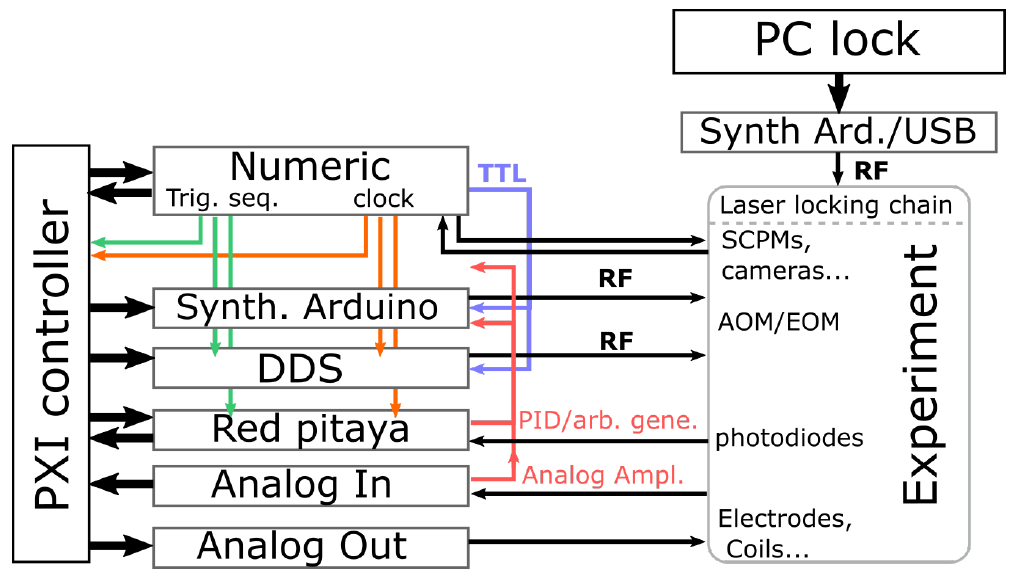
\includegraphics[width=0.5\columnwidth]{images/chapter_1/control.png}
    \caption{Control of the experiment (image extracted from \cite{julien}).}
    \label{fig:ch1_control}
\end{figure}

A schematic of the experimental control system is shown in Figure \ref{fig:ch1_control}. It consists of a PXI (PCI eXtensions for Instrumentation) system that sends instructions to different cards; various instruments synchronized by a trigger signal generated by the numeric card; Arduino channels that produce RF (radio frequency) signals that control laser beams; digital channels that control RF channels, cameras, etc; analog outputs that control RF signals, electrode voltages, etc; analog inputs that record photodiode signals from 100 kHz to 250 MHz; and more.

A photograph of an examlpe PXI system is shown in Figure \ref{fig:ch1_chassis}, which is a National Instrument (NI) PXIe-1078 chassis with the three main modules of interest built-in: NI PXI-6713 Analog Output, NI 5761 Analog Input, and NI 6581 Digital I/O.

\begin{figure}[ht]
    \centering
    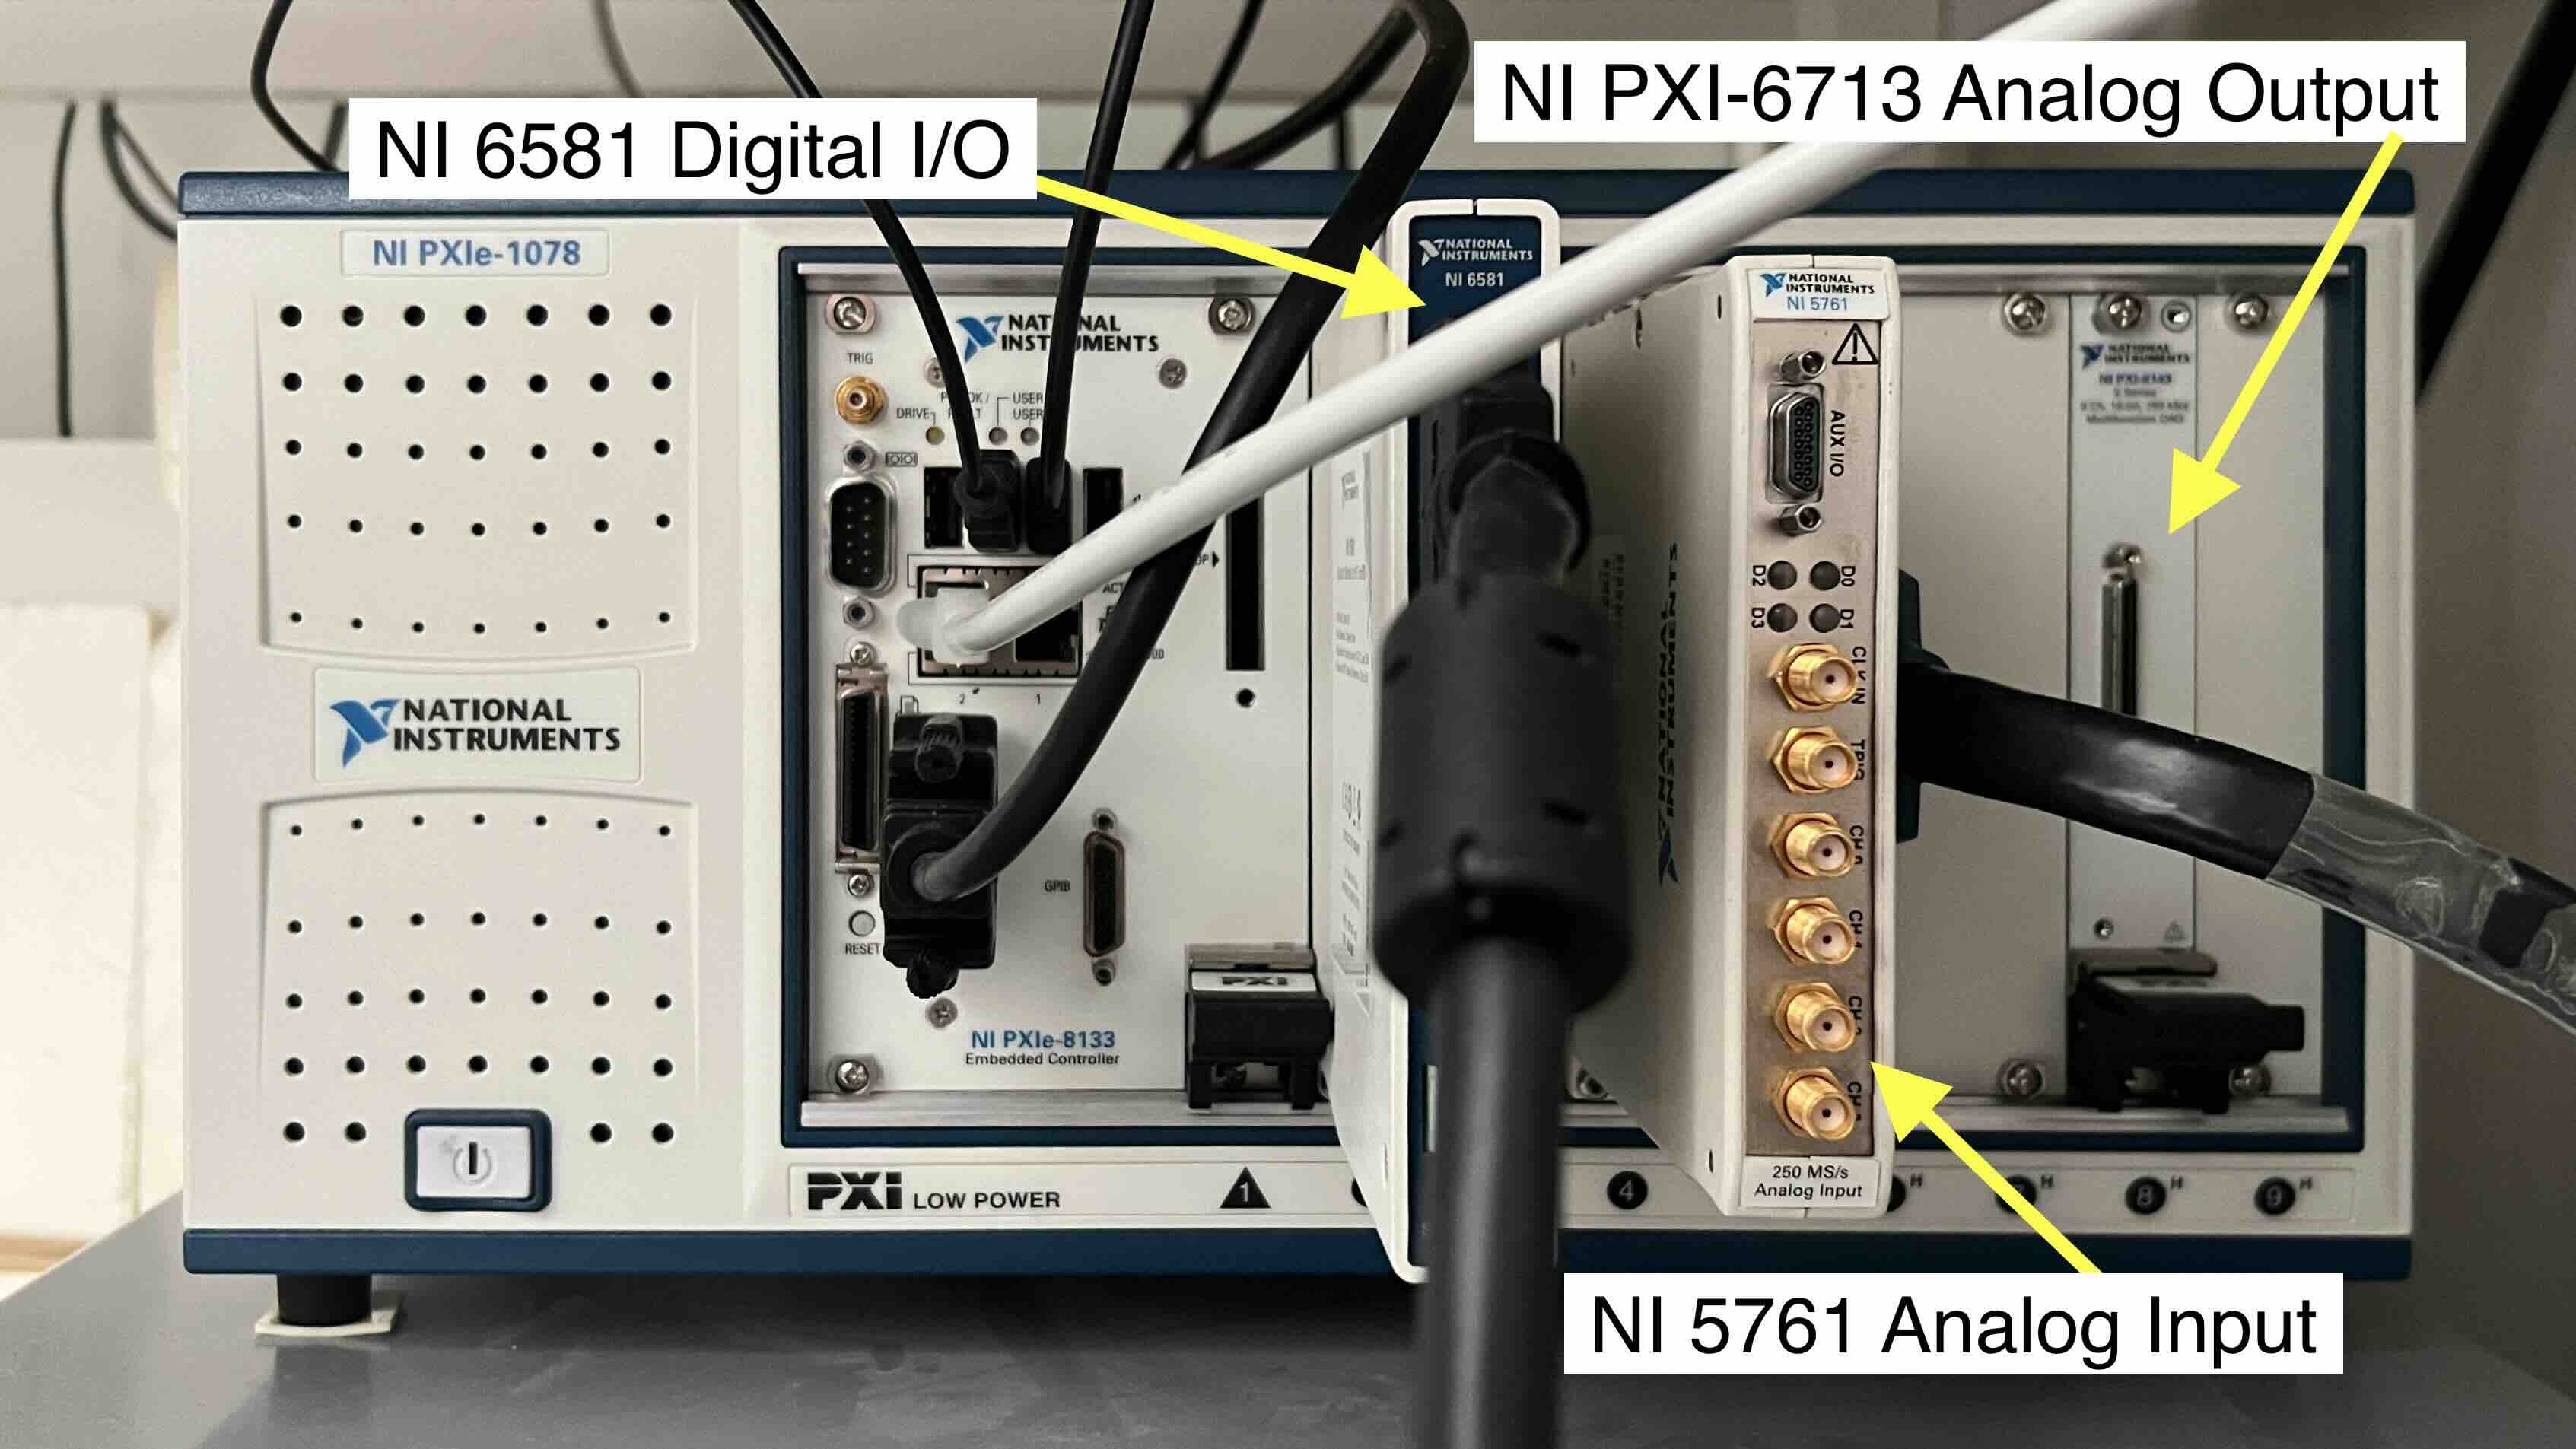
\includegraphics[width=0.6\columnwidth]{images/chapter_1/chassis.jpeg}
    \caption{An NI PXIe-1078 chassis equipped with the three modules used in the experiment for digital and analog inputs/outputs.}
    \label{fig:ch1_chassis}
\end{figure}

%%%%%%%%%%%%%%%%%%%%%%%%%%%%%%%%%%%%%%%%%%%%%%%%%%%%%%%%%%%%%%%%%%%%%%%%%%%%%%%%
\subsection{Software}

The main control of the platform is executed through a home-made LabVIEW program (VITO) on the PXI system. The program's interface is separated into four main panels: \textit{Select Channels}, \textit{Config Sequence}, \textit{Config Channels}, and \textit{Run Sequence}. A screenshot of the \textit{Config Channels} panel of the VITO program interface is shown in Figure \ref{fig:ch1_vito_channels}.

\begin{figure}[ht]
    \centering
    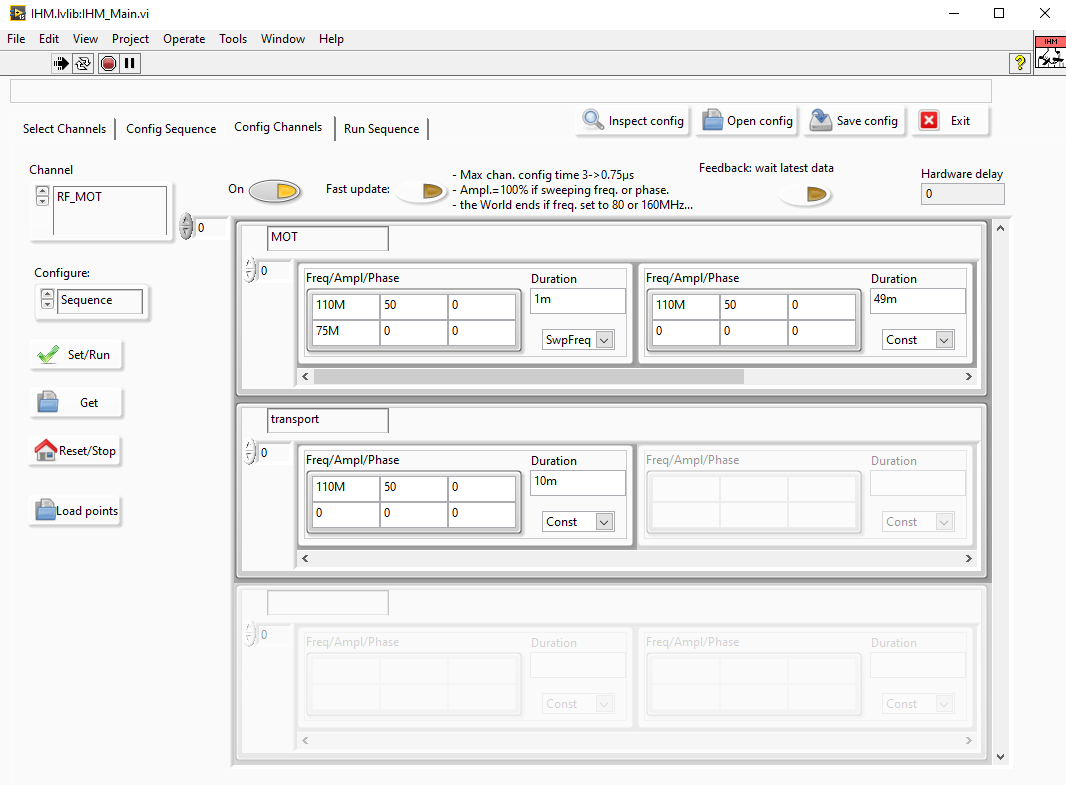
\includegraphics[width=0.98\columnwidth]{images/chapter_1/vito_channels.png}
    \caption{VITO, Config Channels.}
    \label{fig:ch1_vito_channels}
\end{figure}


